\documentclass[12pt,a4paper]{article}
\usepackage{kotex}
\usepackage{graphicx}
\usepackage{hyperref}
\usepackage{indentfirst}
\usepackage{subcaption}
\usepackage{multirow}
\usepackage{flafter}
\usepackage{tikz}
\usetikzlibrary{arrows.meta, intersections, decorations.markings,
    positioning, backgrounds, through, calc, angles, quotes}
\usepackage{amsmath}
\usepackage[top=3cm, bottom=2.54cm, left=2.54cm, right=2.54cm]{geometry}
\usepackage[yyyymmdd]{datetime}
\renewcommand{\dateseparator}{-}
\usepackage{array}
\newcolumntype{L}[1]{>{\raggedright\let\newline\\\arraybackslash\hspace{0pt}}m{#1}}
\newcolumntype{C}[1]{>{\centering\let\newline\\\arraybackslash\hspace{0pt}}m{#1}}
\newcolumntype{R}[1]{>{\raggedleft\let\newline\\\arraybackslash\hspace{0pt}}m{#1}}

\begin{document}
\begin{titlepage}
    \centering
    \begin{tabular}{|C{15cm}|}
        \hline
        \rule{0in}{6ex}
        {\huge 물리학 및 실험 1\par} \\ 
        {\large $^{\textrm{스마트 카트를 활용한}}$뉴턴의 운동 제2법칙\par} \\
        \hline
    \end{tabular} \\
    \vspace{5cm}
    \includegraphics[height=7.36cm]{logo.png}\par
    \vspace{3cm}
    \begin{tabular}{|l|l|l|l|l|l|}
        \hline
        과목 & \multicolumn{5}{l|}{물리학및실험1} \\
        \hline
        담당교수 & \multicolumn{2}{l|}{전계진} & 담당조교 & \multicolumn{2}{l|}{} \\
        \hline
        조 및 조원 & \multicolumn{5}{l|}{2조, 김민수 김민규 김민서 김백준 김연주} \\
        \hline
        제출일 & \multicolumn{5}{l|}{\today} \\
        \hline
        작성자 & 김민수 & 학번 & 20518009 & 학과 & 정보보호 \\
        \hline
    \end{tabular}
\end{titlepage}
이 실험은 뉴턴의 운동 제2법칙을 확인하는 실험이다. 뉴턴의 운동 제2법칙은 "물체에 힘이
작용하면 물체는 가속되는데, 이 때 생긴 가속도는 물체에 가한 힘의 크기에 비례하고,
물체의 질량에 반비례한다" 는 것이다.

우리는 역한트랙 위에서 수레를 가속시키는 실험을 할 것이다. 수레의 질량과 수레를 끄는
힘의 크기를 바꾸어가면서 가속도와 힘, 그리고 가속도와 질량 사이의 관계를 조사할 것이다.

우리는 이 실험에서 스마트카트를 수레를 사용할 것이다. 스마트카트에는 무선으로 동작하는
위치, 속도, 가속도, 힘 센서가 내장되어 있어서 시간에 따른 카트의 위치, 속도, 가속도가
자동으로 기록된다. 우리는 역학 트랙 위에서 스마트카트를 가속 운동시키면서 시간에 따른
물체의 위치, 속도, 가속도를 측정하여 뉴턴의 운동법칙이 성립하는지를 확인한다.
\section{실험목적}
추와 도르래를 이용하여 수레(스마트 카트)를 가속시킬 때 뉴턴의 운동 제2법칙이
성립하는지 살펴본다. 다시 말해 수레를 끄는 힘과 가속도, 그리고 질량과의 관계를
확인해본다.
\section{실험원리}
그림~\ref{fig1-a}과 같이 도르래에 걸쳐진 줄에 연결된 A과 B의 운동을 생각해보자.
\begin{figure}
    \centering
    \begin{subfigure}[]{0.3\textwidth}
        \centering
            \includegraphics[height=4.36cm]{pulley.png}
        \caption{\label{fig1-a}}
    \end{subfigure}
    \begin{subfigure}[]{0.3\textwidth}
        \centering
        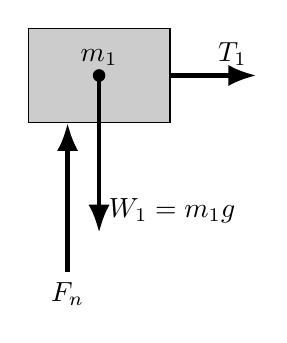
\begin{tikzpicture}
            \fill[gray!40, draw=black] (-0.9, -0.6) rectangle (0.9, 0.6);
            \fill[black] (0, 0) circle(0.08);
            \node[above] at (0, 0) {$m_1$};
            \draw[-{Latex}, ultra thick] (0, 0) -- (0, -2);
            \node[above right] at (0, -2) {$W_1=m_1g$};
            \draw[-{Latex}, ultra thick] (-0.4, -2.5) -- (-0.4, -0.6);
            \node[below] at (-0.4, -2.5) {$F_n$};
            \draw[-{Latex}, ultra thick] (0.9, 0) -- (2, 0);
            \node[above left] at (2, 0) {$T_1$};
        \end{tikzpicture}
        \caption{\label{fig1-b}}
    \end{subfigure}
    \begin{subfigure}[]{0.3\textwidth}
        \centering
        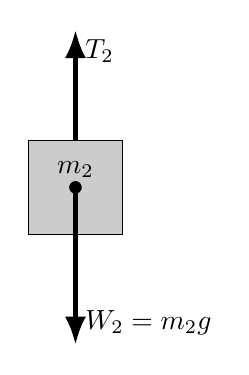
\begin{tikzpicture}
            \fill[gray!40, draw=black] (-0.6, -0.6) rectangle (0.6, 0.6);
            \fill[black] (0, 0) circle(0.08);
            \node[above] at (0, 0) {$m_2$};
            \draw[-{Latex}, ultra thick] (0, 0) -- (0, -2);
            \node[above right] at (0, -2) {$W_2=m_2g$};
            \draw[-{Latex}, ultra thick] (0, 0.6) -- (0, 2);
            \node[below right] at (0, 2) {$T_2$};
        \end{tikzpicture}
        \caption{\label{fig1-c}}
    \end{subfigure}
    \caption{\label{fig1} 줄로 연결된 두 물체의 운동. 수직으로 매달린 물체의 무게
        $(m_2g)$에 의해 두 물체(질량$=m_1+m_2$)가 가속된다.}
\end{figure}
이 때, A와 B의 질량을 각각 $m_1$과 $m_2$, 가속도를 각각 $a_1$과 $a_2$, 줄에 걸리는
장력을 각각 $T_1$과 $T_2$라고 하고, 만약 $a_1$이 $m_1$의 수평성분이라면
뉴턴의 제2법칙은 식~\ref{eq1}과 같다.
\begin{equation}
    \begin{aligned}
        T_1 = m_1a_1
        \label{eq1}
    \end{aligned}
\end{equation}

매달려있는 B의 가속도는 아래쪽 방향이다. B에 작용하는 힘은 아래쪽으로 향하는 중력
$m_2$와 위로 향하는 장력 $T_2$가 있다. 만약 B의 가속도 $a_2$의 아래쪽 방향을 양(+)
으로 택하면 뉴턴의 제2법칙은 식~\ref{eq2}과 같이 된다.
\begin{equation}
    \begin{aligned}
        m_2g-T_2=m_1a_2
        \label{eq2}
    \end{aligned}
\end{equation}

만약 줄의 질량과 도르래의 마찰을 무시한다면, 줄에 걸리는 장력 $T_1=T_2\equiv T$가
된다. 또 연결된 줄이 늘어나거나 줄어들지 않는다고 가정한다면, 두 물체는 똑같은
속력으로 움직여서 $a_1=a_2\equiv a$가 된다. 따라서 위의 두 식은 식~\ref{eq3},
식~\ref{eq4}과 같이 바꾸어 쓸 수 있다.
\begin{equation}
    \begin{aligned}
        T=m_1a
        \label{eq3}
    \end{aligned}
\end{equation}
\begin{equation}
    \begin{aligned}
        m_2g-T=m_2a
        \label{eq4}
    \end{aligned}
\end{equation}

식~\ref{eq3}, 식~\ref{eq4}에서 $T$를 소거하면
$$m_2g-m_1a=m_2a$$

즉
\begin{equation}
    \begin{aligned}
        a=\frac{m_2g}{(m_1+m_2)}
        \label{eq5}
    \end{aligned}
\end{equation}

우리는 이 실험에서 전체 계에 작용하는 힘($F=m_2g$) 또는 전체 계의 질량($m_1+m_2$)을
변화시켜서, 가속도(a)가 힘 또는 질량과 어떤 관계가 있는지 알아볼 것이다.
\section{실험장치}
이 실험에 필요한 실험 장치 및 기구는 다음과 같다.
\subsection{역학 실험장치}
- 역학 트랙, 풀리(도르래), 수평계, 고무줄 탄성 범퍼, 자기 범퍼, 트렉 마운트

- 추걸이, 추 세트 (질량 10g, 50g, 500g, 20g $\times$ 2개), 실(3m)
\subsection{센서 실험장치}
- 컴퓨터, PASCO 550 Universal Interface, 데이터 수집 킻 분석 소프트웨어(Capstone)

- 스마트 카트 (카트 범퍼)

\subsubsection{역학 트랙(Dynamics Track. ME-9779)}
역학트랙은 카트의 직선운동 실험을 수행하기 위한 트랙으로, 길이 2.2m의 알루미늄 트랙과
높이와 수평을 조정할 수 있는 두 개의 트랙 받침으로 구성된다. 그리고 트랙 옆면에서는
파인 홈이 만들어져 있어 카트 범퍼를 고정하거나 다른 센서를 고정하는데 이용할 수 있다.
\begin{figure}
    \centering
    \includegraphics[height=4.36cm]{kinetic_track.jpg}
    \caption{\label{fig2} 역학트랙. 카트의 직선운동 실험을 수행하기 위한 트랙이다.}
\end{figure}

\subsubsection{스마트 카트(Smart Cart. ME-1240 \& ME-1241)}
스마트 카트는 센서가 내장된 역학수레로 밑바닥에 4개의 바퀴가 달려있어서 역학
트랙 위에서 거의 마찰없이 활주할 수 있다. 내부에는 위치, 속도, 가속도, 힘을 측정하는
센서가 내장되어 있어서 블루투스를 통해서 무선으로 데이터를 전송할 수 있다. 뉴턴의
운동법칙을 비롯하여 다양한 역학 실험에서 활용될 수 있다.
\begin{figure}
    \centering
    \begin{subfigure}[]{0.4\textwidth}
        \centering
        \includegraphics[height=4.36cm]{ME-1241.png}
    \end{subfigure}
    \begin{subfigure}[]{0.4\textwidth}
        \centering
        \resizebox{8cm}{!}{
            \begin{tabular}{l l l}
                \hline
                \multirow{4}{*}{힘}     & 측정범위 & $\pm$100N \\
                \cline{2-3}
                                        & 정확도 & $\pm$2\% \\
                \cline{2-3}
                                        & 해상도 & 0.1N \\
                \cline{2-3}
                                        & 최대 샘플링 비율 & 500Hz \\
                \hline
                위치                    & 해상도 & $\pm$0.2mm \\
                \hline
                \multirow{2}{*}{속도}   & 최대속도 & $\pm$3m/s \\
                \cline{2-3}
                                        & 최대 샘플링비율 & 100Hz \\
                \hline
                \multirow{2}{*}{가속도} & 측정범위 & $\pm16g$ ($g=9.8m/s^2$) \\
                \cline{2-3}
                                        & 최대 샘플링비율 & 500Hz \\
                \hline
                블루투스                & 최대 무선범위 & 30m(장애물이 없을 때) \\
                \hline
            \end{tabular}
        }
        \caption{\label{table1} 스마트 카트에 내장된 센서의 특성}
    \end{subfigure}
    \caption{\label{fig3} 스마트 카트}
\end{figure}
\section{실험 방법}
\subsection{실험 기구 설치}
\begin{enumerate}
    \item 테이블 위에 역학 트랙을 설치하고, 트랙 한쪽 끝에는 자석 범퍼를 설치한다.
        자석 범퍼는 카트가 트랙 밖으로 떨어지는 것을 막아주는 역할을 한다. 이 때
        자석이 보이는 부분이 트랙 한쪽을 향하게 하여 카트가 범퍼에 충돌할 때
        반발하도록 한다. 도르래 쪽 트랙 끝에는 고무줄의 범퍼를 설치하여 카트가 가속될
        때 도르래와 충돌을 막아준다.
    \item 트랙 위에 수평계를 올려놓고, 트랙 앞뒤와 좌우 수평을 맞춘다. 트랙 받침의
        조절나사를 돌려서 수준기로 전후와 좌우의 수평을 맞춘다.
    \item 트랙 위에 카트를 올려놓고 트랙의 수평을 다시 조절한다. 트랙 위에 올려놓은
        카트가 저절로 움직이면, 트랙 다리에 있는 너트를 돌려서 카트가 굴러가지 않도록
        수평을 맞춘다.
    \item 실로 추걸이와 스마트 카트를 연결하여 실을 도르래에 걸어준다. 실이 트랙과
        평행하도록 도르래의 높이를 조정한다.
    \item 카트를 트랙 위에서 움직여 보고, 카트가 트랙 끝에 도달하기 위해 추가 바닥에
        부딪히지 않도록 실의 길이를 조절한다.
\end{enumerate}
\subsection{센서와 캡스톤 프로그램 설정}
\begin{enumerate}
    \item 캡스톤 프로그램을 실행한다.
    \item 스마트 카트를 연결하고 스마트 카트에 내장된 센서(위치, 속도, 가속도)를
        설정한다. 각 센서 아이콘을 선택한 후 [Properties] 아이콘을 클릭한다. 시간에
        따른 카트의 위치, 속도, 가속도를 측정한다.
    \item \label{par1} 측정 자동 완료 조건을 구성한다. [Controls] 메뉴에서
        [Recording Conditions]을 클릭하여 나타난 화면에서 카트가 0.5m 이동하면
        자동으로 측정이 완료되도록 구성한다.
    \item 위~\ref{par1}의 설정에 의해 측정이 정상적으로 완료되는지 확인한다. 실험
        진행되기 전 초기 화면에는 [Record]버튼이 보이지만 [Record]를 클릭하면 [Stop]
        버튼으로 바뀌고, 초시계 하단에 [Recording]이 표시되면서 데이터 측정이
        시작된다. 카트가 0.5m 이동하면 (카트의 회전운동센서에서 측정된 변위값이 0.5m
        가 되면) 자동으로 측정이 종료된다.
    \item 단위 시간당 데이터 측정 횟수를 설정한다. 힘 센서와 회전운동센서 모두 1초에
        50회(50Hz)로 데이터를 측정한다. 모든 센서에 대해 동일한 값으로 설정해야 한다.
    \item {[Display] 팔레트에서 [Graph] 아이콘을드래그하여 그래프를 생성한다.
        화면 우측에 있는 [Displays]팔레트에서 [Graph]아이콘을 화면 중앙으로
        드래그하면 그래프 창이 나타난다. 그래프 상단의 메뉴에서
        [Add new plot area ... ]를 클릭하여 $X$축이 동기화된 그래프를 2개 더
        추가한다. 그래프 창에서 <Select Measurment>를 클릭한 후, $x$축으로
        [Time(s)], $y$축으로 각각 [Position(m)], [Velocity(m/s)], 
        [Acceleration (m/s$^2$)]를 선택한다.}
\end{enumerate}
\subsection{순간 속도와 평균속도}
역학 트랙 위에서 스마트 카트를 움직이게 하고, 시간에 따른 위치와 속도, 가속도를
기록한다. 그리고 이 결과를 비교하여 순간속도와 평균속도가 어떻게 다른지 비교 분석한다.
\begin{enumerate}
    \item 카트의 질량을 측정하고 기록한다. 전자저울을 사용하여 카트와 카트에 실린
        무게추의 질량을 함께 측정한다.
    \item 추걸이와 추의 질량을 측정하고 기록한다.
    \item 카트의 출발 위치를 결정한다. 카트를 트랙 위에 올려놓은 후, 추걸이가 도르래
        근처에 도달할 때까지 카트를 뒤로 당긴다.
    \item 카트를 뒤쪽으로 0.5m정도 잡아당긴 다음 가만히 붙들고 있는다. 출발 지점을
        표시해 두고 같은 지점에서 출발시키는 방법을 사용할 수도 있다.
    \item 캡스톤 프로그램에서 [Record]버튼을 클릭하여 데이터 측정을 시작한다.
    \item 붙들고 있던 카트를 가만히 놓아준다. 추의 무게에 의해 카트가 천천히
        가속된다. 카트가 종료 조건에서 설정한 거리(0.5m)를 지나면 자동으로 측정이
        중단된다.
    \item 실험 결과를 분석한다.
\end{enumerate}
\subsection{끄는 힘의 크기 변화에 따른 가속 운동}
전체 질량($m_1+m_2\equiv m$)을 고정하고, 끄는 힘($F=m_2g$)을 바꾸어가며 실험한다.
다시 말해 카트($m_1$)에 있던 무게 추를 하나씩 차례로 $m_2$로 옮기면서
($m_1+m_2=$일정) 가속 실험을 되풀이한다.
\begin{enumerate}
    \item 도르래를 제외한 계의 전체 질량, 즉 (수레+수레하중+추걸이+추)의 질량을
        기록하라.
    \item \label{par2}먼저 수레 위에 있는 추 하나(10g)를 추걸이로 옮긴 다음
        스마트카트를 추걸이가 도르래에 닿지 않을 정도로 최대한 잡아당긴다.
    \item \label{par3}캡스톤 [Record] 버튼을 클릭하여 기록을 시작하고, 수레를
        출발시킨다.
    \item 손을 놓은 후 엔드스탑에 충돌하기 전까지의 가속도의 그래프를 얻고, 툴을
        이용하여 평균을 계산하여 표에 기록한다.
    \item 카트의 추를 도르래로 옮겨(총 질량 고정) 추걸이에 걸린 질량을 10g단위로
        늘려가면서 \ref{par2}$\sim$\ref{par3}과정을 반복한다. (총 5회)
\end{enumerate}
\subsection{물체의 질량 변화에 따른 가속 운동}
끄는 힘($F=m_2g$)을 일정하게 하고, 전체 질량($m_1+m_2$)을 바꾸어가며 실험한다. 다시
말해 $m_2$의 질량을 일정하게 하고, $m_1(m_1+m_2\equiv m)$의 질량을 변화시켜가면서
가속 실험을 한다.
\begin{enumerate}
    \item 도르래에 20g추를 걸고 스마트카트에는 추를 올리지 않는다.
    \item \label{par4}스마트카트를 추걸이가 도르래에 닿지 않을 정도로 최대한 잡아당긴
        후 놓아 가속도를 측정한다.
    \item \label{par5}손을 놓은 후 엔드스탑에 충돌하기 전까지의 가속도의 그래프를
        얻고, 툴을 이용하여 평균을 계산하여 표에 기록한다.
    \item 스마트카트에 올린 추의 질량을 50g씩 늘려 \ref{par4}$\sim$\ref{par5}과정을
        반복한다. (총 5회)
\end{enumerate}
\section{실험 결과 및 분석}
\subsection{실험 1}
Figure~\ref{fig4}참조
\begin{figure}
    \centering
    \includegraphics[width=15cm]{week7pos.png}
    \includegraphics[width=15cm]{week7vel.png}
    \includegraphics[width=15cm]{week7acc.png}
    \caption{\label{fig4}시간에 따른 물체의 운동 그래프}
\end{figure}
\subsection{실험 2}
Figure~\ref{fig5}를 보면, a와 F의 의 관계를 나타내는 그래프이고. $F=ma$이기 떄문에
$a$가 증가함에 따라 질량 $m$은 고정되었으므로, $F$또한 비례하게 증가하는 것을
알 수 있다.
\begin{figure}
    \centering
    \begin{tabular}{|c|c|c|c|c|}
        \hline
        \multirow{2}{*}{
                \begin{tabular}{@{}c@{}}
                    (수레+추)의 질량\\
                    $m_1$[$g$]
                \end{tabular}
            } & \multirow{2}{*}{
                \begin{tabular}{@{}c@{}}
                    (추걸이+추)의 질량\\
                    $m_2$[$g$]
                \end{tabular}
            } & \multicolumn{3}{c|}{가속도} \\
        \cline{3-5}
        && $a_{\textrm{측정}}$ [$m/s^2$] & $a_{\textrm{계산}}$ [$m/s^2$] & 오차 \\
        \hline
        수레+170 & 5 & 0.104 & 0.115 & 0.011 \\
        \hline
        수레+160 & 15 & 0.332 & 0.346 & 0.014 \\
        \hline
        수레+150 & 25 & 0.556 & 0.576 & 0.020 \\
        \hline
        수레+140 & 35 & 0.790 & 0.807 & 0.017 \\
        \hline
        수레+130 & 45 & 1.004 & 1.038 & 0.034 \\
        \hline
    \end{tabular}
    \includegraphics[width=16.2cm]{week7af.png}
    \caption{\label{fig5}}
\end{figure}
\subsection{실험 3}
Figure~\ref{fig6}을 보면, 질량과 가속도는 반비례하는 관계임을 알 수 있는데, 이는
$F=ma$ 식에 미루어 보면, 같은 힘으로 잡아당길 떄 $F$ 값이 고정되고, 이에 따라 질량이
늘어나면 가속도가 줄 수밖에 없는 반비례관계가 성립함을 알 수 있다. 그러므로
실제 결과로 보아도, 식으로만 보아도, 반비례함을 알 수 있다.
\begin{figure}
    \centering
    \resizebox{16.2cm}{!}{
        \begin{tabular}{|l|c|c|c|c|c|}
            \hline
            \multirow{2}{*}{
                \begin{tabular}{@{}c@{}}
                    (수레+추)의 질량\\
                    $m_1$[$g$]
                \end{tabular}
            } & \multirow{2}{*}{
                \begin{tabular}{@{}c@{}}
                    (추걸이+추)의 질량\\
                    $m_2$[$g$]
                \end{tabular}
            } & \multirow{2}{*}{
                \begin{tabular}{@{}c@{}}
                    전체 질량$m$\\
                    $m_1 + m_2$[$g$]
                \end{tabular}
            } & \multicolumn{3}{c|}{가속도} \\
            \cline{4-6}
            &&& $a_{\textrm{측정}}$ [$m/s^2$] & $a_{\textrm{계산}}$ [$m/s^2$] & 오차 \\
            \hline
            수레 & 25 & 275 & 0.841 & 0.817 & -0.024 \\
            \hline
            수레+50 & 25 & 325 & 0.709 & 0.700 & -0.009 \\
            \hline
            수레+100 & 25 & 375 & 0.616 & 0.613 & -0.003 \\
            \hline
            수레+150 & 25 & 425 & 0.542 & 0.544 & 0.002 \\
            \hline
            수레+200 & 25 & 475 & 0.481 & 0.490 & 0.009 \\
            \hline
        \end{tabular}
    }
    \includegraphics[width=16.2cm]{week7am.png}
    \caption{\label{fig6}}
\end{figure}
\section{실험 고찰}
\subsection{실험1:a-스마트 카트가 주행하는 동안 카트의 위치, 순간속도와 가속도는 각각
    어떤 양상인가?}
스마트 카트가 주행하는 동안 카트는 추에 의해 일정한 힘으로 가속하게 된다. 그러므로
위치는 점점 빠르게 멀어지고, 순간속도도 점점 빨라진다. 그러나 카트에 가하는 힘이
일정하므로 가속도도 일정하게 유지된다.
\subsection{실험1:b-스마트 카트의 운동은 어떤 운동인가?}
도르래와 도르래 축과의 마찰력, 실과 도르래의 마찰, 공기저항, 수레 바퀴와 바퀴 축과의
마찰력을 무시한다면 가속도가 일정하게 유지되는 운동이므로, 등가속도 운동으로 볼 수
있다. 또한 시간에 대한 위치 그래프를 보면 위치가 2차함수의 꼴로 증가하기 때문에
등가속도라고도 볼 수 있다.
\subsection{실험2:끄는 힘(F)과 가속도(a)사이에는 어떤 관계가 있는가? (엑셀을 이용하여
    추세선을 구해서 F와 a사이에 어떤 비례 관계가 있는지 보고 판단하라)}
\begin{figure}
    \centering
    \includegraphics[width=14.2cm]{week7af.png}
    \caption{\label{fig7}}
\end{figure}
Figure~\ref{fig7}을 보면, $F=ma$ 식에 따라 운동하므로 전체 질량 $m$이 변하지 않는
상황에서 가속도가 변하면 힘 또한 비례하게 바뀐다. 이 떄 비례하는 숫자가 $m$이므로
질량에 따라 비례한다. 그러나 실제 측정 데이터를 보면, a-F그래프의 추세선 기울기가
0.4339 이기 때문에 실제로 질량값인 0.425에 비례하진 않는다. 하지만 오차가 0.02 미만인
아주 비슷한 값에 비례하는 것을 알 수 있다.
\section{오차 원인}
Figure~\ref{fig7}을 보면, 질량(=0.425)에 비례해야 하고 (0, 0)을 지나야 할
그래프이지만 그래프의 식을 보면 0.4339에 비례하고 (0, 0.0032)를 지나는 걸 알 수 있다.
이렇게 되는 원인으로는 도르래의 마찰, 수레 바퀴의 마찰, 공기의 저항 등의 이유가 있을
것 같다. 그리고 이를 줄이기는 현실적으로 어려워 보이기에 다른 실험을 통해 관계식을
알아내어 보정하는 것이 바람직 해 보인다. 그리고 Figure~\ref{fig4}의 위치-시간
그래프를 보면 마지막 5개 측정값이 이상한데, 이는 아무래도 스마트 카트의 통신 과정에서
값을 두 번 수신받은 것으로 보이며, 그 증거로는 마지막 5개 데이터와 마지막 5개 데이터
앞 5개 데이터가 완전히 일치한다. 해결 방안으로는 마지막 5개 데이터를 무시하는 것이
좋아 보인다. 그리고 Figure~\ref{fig4}에서의 가속도 그래프를 보면 값이 요동치는 것으로
보이는데. 이는 가속도 센서의 오차로 인한 것으로 보이나, 그 값의 변동이 $\pm$0.04
정도로 매우 작아 보이므로, 평균을 냄으로써 무시해도 될 수준인 것 같다.
\section{실험을 통해 배우게 된 것}
\begin{itemize}
    \item $F=ma$가 생각보다 마찰력이나 공기저항에 대해 크게 차이나지 않는다는 점.
    \item $a-F$ 그래프가 질량에 비례한다는 것을 알았다.
\end{itemize}
\section{실험원리의 실생활에서의 예}
\begin{itemize}
    \item 에베레스트 등산가들끼리 뭄을 묶고 산을 등반할 때 한 사람이 절벽으로 떨어진
        상황이다. 이 때 모든 사람에게 떨어진 사람의 무게 만큼의 힘이 작용한다. 하지만
        유감스럽게도 이 실험에서는 등반가의 발에 바퀴가 달려있으므로 모두가 같이
        떨어지고 있다.
    \item etc..
\end{itemize}
\end{document}